%%%%%%%%%%%%%%%%%%%%%%%%%%%%%%%%%%%%%%%%%%%%%%%%%%%%%%%%%%%%%%%
%
% Welcome to Overleaf --- just edit your LaTeX on the left,
% and we'll compile it for you on the right. If you open the
% 'Share' menu, you can invite other users to edit at the same
% time. See www.overleaf.com/learn for more info. Enjoy!
%
%%%%%%%%%%%%%%%%%%%%%%%%%%%%%%%%%%%%%%%%%%%%%%%%%%%%%%%%%%%%%%%

% Inbuilt themes in beamer
\documentclass{beamer}

%packages:
% \usepackage{tfrupee}
% \usepackage{amsmath}
% \usepackage{amssymb}
% \usepackage{gensymb}
% \usepackage{txfonts}

% \def\inputGnumericTable{}

% \usepackage[latin1]{inputenc}                                 
% \usepackage{color}                                            
% \usepackage{array}                                            
% \usepackage{longtable}                                        
% \usepackage{calc}                                             
% \usepackage{multirow}                                         
% \usepackage{hhline}                                           
% \usepackage{ifthen}
% \usepackage{caption} 
% \captionsetup[table]{skip=3pt}  
% \providecommand{\pr}[1]{\ensuremath{\Pr\left(#1\right)}}
% \providecommand{\cbrak}[1]{\ensuremath{\left\{#1\right\}}}
% %\renewcommand{\thefigure}{\arabic{table}}
% \renewcommand{\thetable}{\arabic{table}}      

\setbeamertemplate{caption}[numbered]{}

\usepackage{enumitem}
\usepackage{tfrupee}
\usepackage{amsmath}
\usepackage{amssymb}
\usepackage{gensymb}
\usepackage{graphicx}
\usepackage{txfonts}

\def\inputGnumericTable{}

\usepackage[latin1]{inputenc}                                 
\usepackage{color}                                            
\usepackage{array}                                            
\usepackage{longtable}                                        
\usepackage{calc}                                             
\usepackage{multirow}                                         
\usepackage{hhline}                                           
\usepackage{ifthen}
\usepackage{caption} 
\captionsetup[table]{skip=3pt}  
\providecommand{\pr}[1]{\ensuremath{\Pr\left(#1\right)}}
\providecommand{\cbrak}[1]{\ensuremath{\left\{#1\right\}}}
\renewcommand{\thefigure}{\arabic{table}}
\renewcommand{\thetable}{\arabic{table}}   
\providecommand{\brak}[1]{\ensuremath{\left(#1\right)}}
\providecommand{\brak}[1]{\ensuremath{\left(#1\right)}}

% Theme choice:
\usetheme{CambridgeUS}

% Title page details: 
\title{Assignment 9} 
\author{Vedant Bhandare (cs21btech11007)}
\date{May 2022}
\logo{\large \LaTeX{}}

\begin{document}

% Title page frame
\begin{frame}
    \titlepage 
\end{frame}

% Remove logo from the next slides
\logo{}


% Outline frame
\begin{frame}{Outline}
    \tableofcontents
\end{frame}

% Lists frame
\section{Question}
\begin{frame}{Question}
    Suppose that the voltage $v$ is a random variable given by $v=i(r+r_0)$, where $i= 0.01$ A, $r_0 = 1000 \Omega$. If the resistance $r$ is a random variable with uniform distribution between $900 \Omega$ and $1100 \Omega$, what is the distribution of the voltage $v$?
\end{frame}

\section{Solution}
\begin{frame}{Distribution of voltage $v$}
    Voltage is given by,
    \begin{align}
        v=i(r+r_0)
    \end{align}
    As resistance $r$ lies between $900 \Omega$ 
    and $1100 \Omega$, voltage $v$ lies between $19 V$ and $21 V$.\\
\end{frame}

\begin{frame}{Formula}
\begin{block}{The probability density function is given by}
    \centering
    $f_Y(y) = \frac{f_X(x_1)}{|g`(x_1)|} + \frac{f_X(x_2)}{|g`(x_2)|} + \frac{f_X(x_3)}{|g`(x_3)|} + ..... + \frac{f_X(x_n)}{|g`(x_n)|}$
\end{block}
    where, $n$ is the number of solutions.
\end{frame}

\begin{frame}
    Consider the equation $y = \frac{1}{x}$. It has a single solution $x = \frac{1}{y}$. Thus, we have,
    \begin{align}
        f_Y(y) = \frac{1}{y^2} f_X(\frac{1}{y})
    \end{align}
\end{frame}

\begin{frame}{Cauchy density}
    \begin{align}
        f_X(x) &= \frac{\alpha / \pi}{x^2 + \alpha^2} \text{is a Cauchy density with parameter $\alpha$}\\
        f_Y(y) &= \frac{1 /\alpha \pi}{y^2 + 1 / \alpha^2} \text{is a Cauchy density with parameter $1 / \alpha$}
    \end{align}
\end{frame}

\begin{frame}
    Consider,
    \begin{align}
        g &= \frac{1}{r}
    \end{align}
        Using (2), we get,
    \begin{align}
        f_g(g) &= \frac{1}{g^2}f_r(r)
    \end{align}
\end{frame}

\section{Graphs}
\begin{frame}{Graphs}
    \centering
    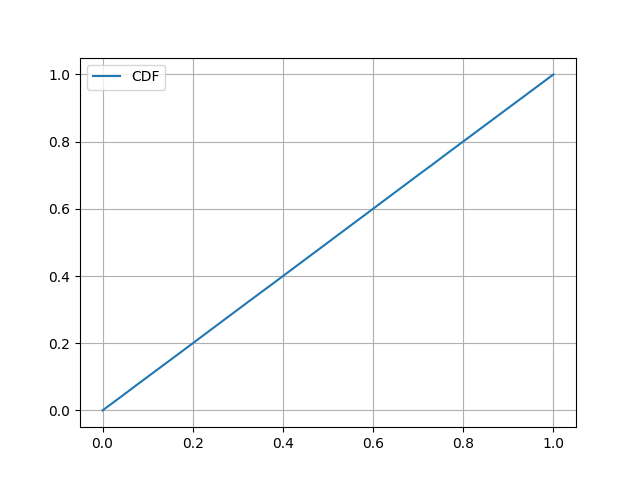
\includegraphics[scale=0.6]{Figure_1.png}
\end{frame}

\begin{frame}{Graphs}
    \centering
    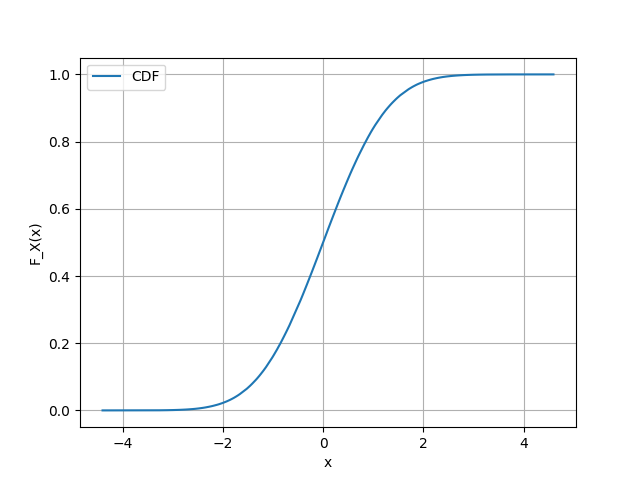
\includegraphics[scale=0.6]{Figure_2.png}
\end{frame}
\end{document}
